\documentclass[11pt, spanish]{article}
\usepackage[utf8]{inputenc}
\usepackage{listings} 
\usepackage{graphicx}
\usepackage{amsfonts}
\usepackage[dvipsnames]{xcolor}
\usepackage[T1]{fontenc}
\usepackage{bigfoot}
\usepackage{amsmath}
\usepackage[numbered,framed]{matlab-prettifier}
\usepackage{caption}
\usepackage[figurename=Figura, tablename=Tabla, font={small,tt}]{caption}
\usepackage{blkarray}
\usepackage{xcolor}
\usepackage{multicol}
\usepackage[]{algorithm2e}
\usepackage{float}
\usepackage[section]{placeins}

\makeatletter
    \setlength\@fptop{0\p@}
\makeatother

\date{}

\usepackage{geometry}
 \geometry{
 a4paper,
 left=30mm,
 right=30mm,
 top=30mm,
 }

\lstset{
	style              = Matlab-editor,
  	basicstyle         = \mlttfamily,
  	escapechar         = ",
  	mlshowsectionrules = true,
	framesep=4.5mm,
	framexleftmargin=2.5mm,
	fillcolor=\color{White},
	rulecolor=\color{Black},
	numberstyle=\normalfont\tiny\color{Black}
}

\captionsetup[lstlisting]{font={small,tt}}
\renewcommand{\lstlistingname}{Script}
\newcommand\RED{\color{red}}
\newcommand\BLUE{\color{blue}}
\newcommand{\BigO}[1]{\ensuremath{\operatorname{O}\bigl(#1\bigr)}}
\newcommand{\norm}[1]{\left\lVert#1\right\rVert}

\begin{document}

\renewcommand\lstlistlistingname{Lista de Scripts}

\author{Sebastián Valencia Calderón \\ 201111578}
\title{Laboratorio 6: Interpolación polinomial.}
\maketitle

%====================================================================
\section{Introducción}

El proceso mediante el cual se toman valores de datos en ciertos puntos es llamado interpolación. En ciertos casos, este problema y la aproximación por interpolación, puede tratarse como un problema de aproximación discreta. La interpolación, puede usarse para construir de manera constructiva ciertas funciones extraídas a partir del comportamiento de datos en $\mathbb{R}^2$, de manera más puntual, proporciona una metodología para la integración numérica, el tratamiento numérico de ecuaciones diferenciales y la discretización de un conjunto más grande de ecuaciones.\\

Los polinomios interpolantes, producto final de la interpolacion polinomial, rara vez son el producto de un proceso numérico, sino mas bien la base para la solución de un conjunto mas amplio de problemas solubles mediante esta metodología. Por lo tanto, estos polinomios aparecen frecuentemente en el análisis y desarrollo de algoritmos numéricos. Dado un conjunto de puntos, se desea explorar el comportamiento de ciertos algoritmos de interpolación, de manera numérica a través de implementaciones de los mismos algoritmos en el lenguaje de programación \textsc{Matlab}. Ademas de los algoritmos, se presenta la solución a problemas aplicados, en los cuales se explora el comportamiento real de los algoritmos, contrastando su comportamiento, y el error generado por la ejecución de los mismos. El desarrollo de estos ejercicios, pretende comprometerse con los siguientes objetivos:

\begin{enumerate}
\item Identificar y entender algunos algoritmos de interpolación con polinomios y Splines.
\item Resolver algoritmos de interpolación mediante el uso de herramientas de computación
matricial disponibles en \textsc{Matlab}.
\item Contrastar la complejidad de implementación y funcionamiento de los algoritmos
implementados.
\end{enumerate}

%==================================================================
\section{Procedimiento}

Para cumplir los objetivos enumerados anteriormente, se implementan tres algoritmos clásicos de interpolación, el de los polinomios interpoladores de Lagrange y el de diferencias de Newton, además, de una variación a los Splines cúbicos naturales, para reducir la oscilación de los polinomios sobre puntos ajenos al conjunto dado como argumento. Con los dos primeros polinomios, se explora un problema de predicción y modelado de datos discretos. Con el ultimo algoritmos, se pretende dibujar una figura con los polinomios resultantes dado un conjunto partido de datos discretos.\\

 El desarrollo de cada uno de estos ejercicios, requiere comprender el funcionamiento y concepto de cada uno de los algoritmos usados para la interpolación de los datos dados. El desarrollo del laboratorio, comienza con la comprensión de cada uno de estos métodos o algoritmos, pero se centra fundamentalmente en la exploración de estos mismos a través de problemas prácticos.

%==================================================================
\section{Resultados}

A continuación, se exponen los resultados, las metodologías propuestas para los análisis y las herramientas de ejecución para cada uno de los problemas propuestos.

\subsection{Implementación de algoritmos en \textsc{Matlab}}

A continuación, se exponen las implementaciones para cada uno de los algoritmos básicos para la interpolación polinomial sobre los datos. Además, se compara cada resultado con la matriz natural, la cual surge al plantear de manera general el problema (esta aproximación, posee todos los problemas sobre representación y dimensionalidad estudiados anteriormente al estudiar la solución de sistemas lineales en un computador).

\subsubsection{Sistema lineal para el polinomio interpolante}

\begin{figure}[H]
\centering
	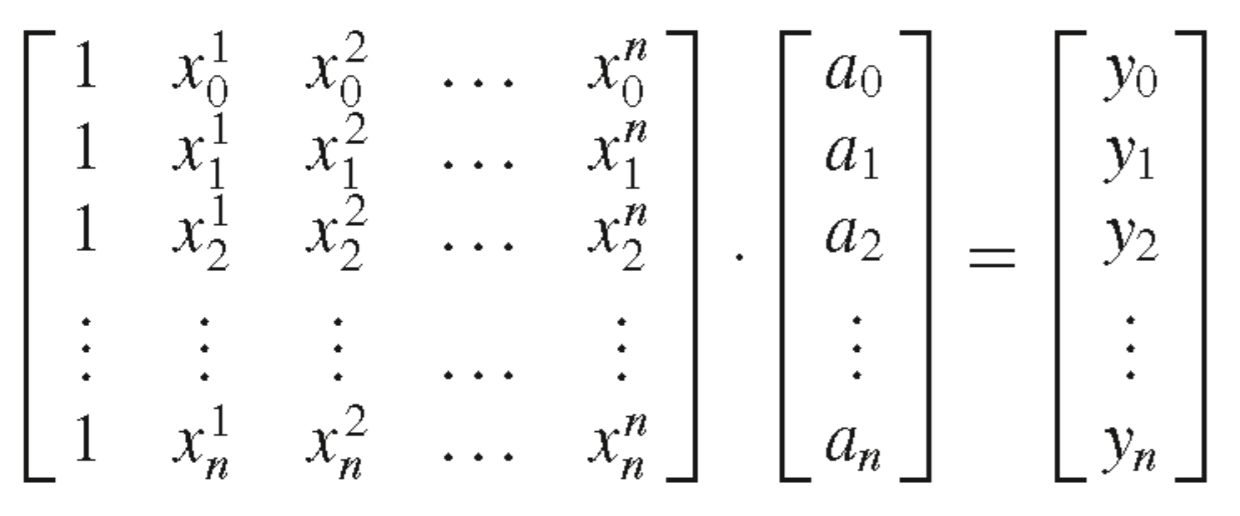
\includegraphics[scale=0.4]{data/img/system}
	\caption{La solución de este sistema lineal, proporciona los coeficientes del polinomio interpolante para un conjunto de datos bi-dimensionales.}
\end{figure}

\lstinputlisting[caption = {Implementación en \textsc{Matlab} del sistema lineal natural para los coeficientes del polinomio interpolante}]{data/scripts/validation.m}\

\subsubsection{Interpolación polinomial de Lagrange}

A continuación, se anexa la funcion en \textsc{Matlab}, que implementa el algoritmo para la obtención de polinomio interpolante de Lagrange. La metodología para este algoritmos, fue estudiada y basada en las de las referencias \cite{yang2005applied} y \cite{burden2010numerical}.

\lstinputlisting[caption = {Implementación en \textsc{Matlab} del polinomio interpolador de Lagrange.}]{data/scripts/lagrange.m}\

\subsubsection{Interpolación polinomial de Newton}

A continuación, se anexa la funcion en \textsc{Matlab}, que implementa el algoritmo para la obtención de polinomio interpolante a partir del metodo de diferencias divididas de Newton-Gregory. La metodología para este algoritmos, fue estudiada y basada en las de las referencias \cite{yang2005applied} y \cite{burden2010numerical}.

\lstinputlisting[caption = {Implementación en \textsc{Matlab} del polinomio de interpolacion haciendo uso el método de diferencias divididas de Newton-Gregory.}]{data/scripts/newton.m}\

\subsubsection{Verificación de la implementación}

Para la validación de los algoritmos frente a la formulación natural del problema, se propone validarlos contra un vector de datos aleatorios, obtener los coeficientes del polinomio interpolante haciendo uso de cada uno de los algoritmos, y obtener el error frente al polinomio obtenido al resolver el sistema lineal. El sistema lineal, es obtenido de acuerdo al esquema mostrado en la figura 1.

\lstinputlisting[caption = {Obtención del sistema lineal para la formulación natural del problema, esto es, de forma matricial.}]{data/scripts/validation.m}\

\lstinputlisting[caption = {Obtención del sistema lineal para la formulación natural del problema, esto es, de forma matricial.}]{data/scripts/verify.m}\

\begin{figure}[H]
\centering
	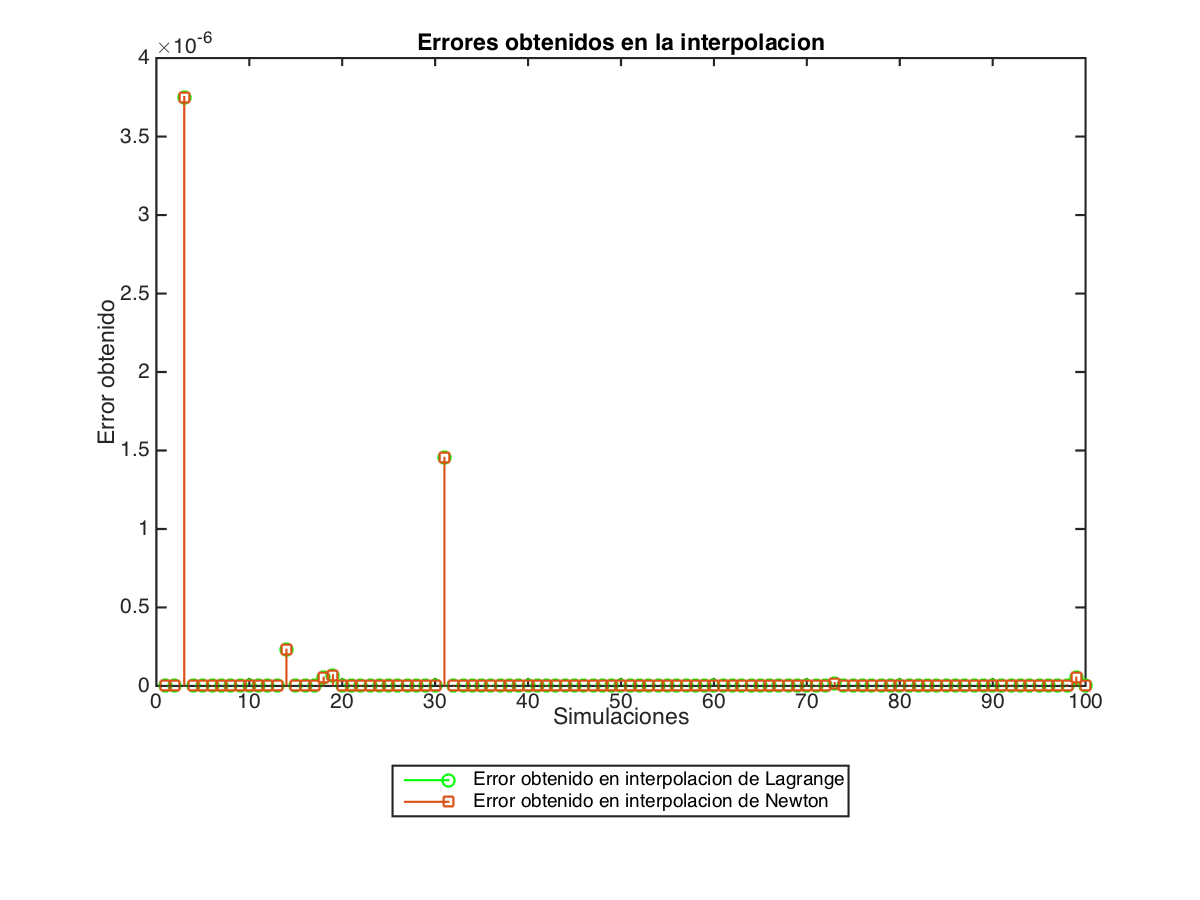
\includegraphics[scale=0.8]{data/img/interpo}
	\caption{El resultado a la simulación, arroja valores alentadores sobre el error obtenido en cada uno de los algoritmos tomando como valor real, la solución del sistema lineal de la formulación general del problema. Puede verse la similitud en resultados de ambos algoritmos, y la baja magnitud del error de cada uno de los algoritmos.}
\end{figure}

\subsection{Problema de aplicacion}

\begin{figure}[H]
\centering
	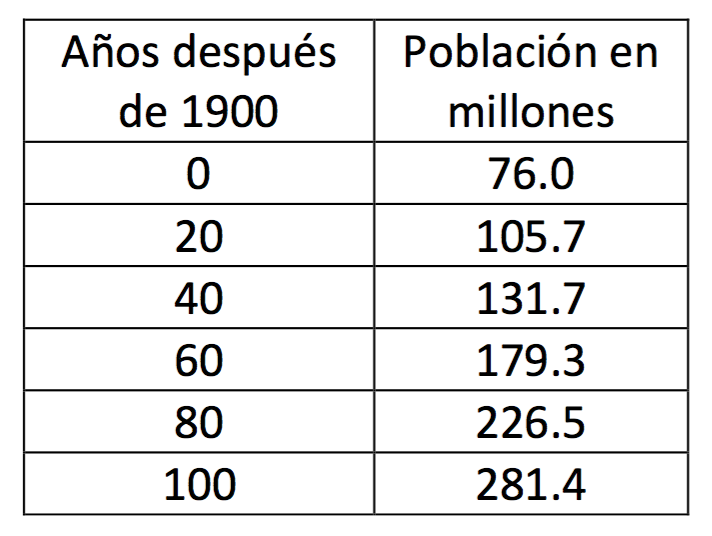
\includegraphics[scale=0.4]{data/img/table}
	\caption{Muestra los datos a usar, el año y la población de Estados Unidos correspondiente a ese año.}
\end{figure}

\begin{itemize}

\item Graficar la población contra el tiempo después de 1900 de acuerdo a la tabla presentada.

\lstinputlisting[caption = {Script para graficar los puntos de población en cada año.}]{data/scripts/population1.m}\

\begin{figure}[H]
\centering
	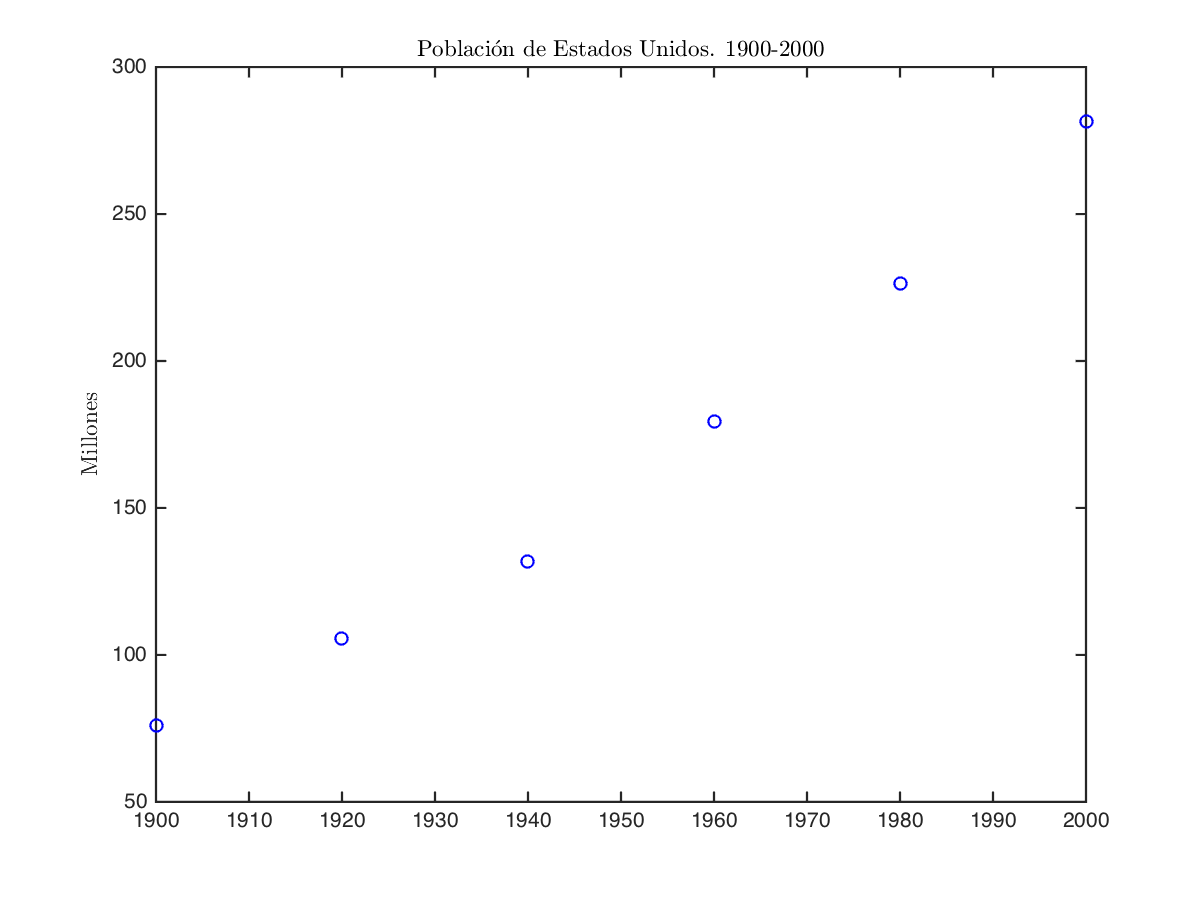
\includegraphics[scale=0.8]{data/img/populationplot}
\end{figure}

\item Encuentre mediante cada uno de los métodos implementados el polinomio de quinto grado que pasa por cada uno de los puntos en la tabla.

\lstinputlisting[caption = {Script para obtener los polinomios de interpolación usando cada método implementado anteriormente.}]{data/scripts/population2.m}\

Los coeficientes de los polinomios obtenidos son:\\

\texttt{lag} $ = $
$$\left(2.0156e-07 \quad -0.00196 \quad 7.6812 \quad -1.4992e+04 \quad 1.4630e+07 \quad -5.7105e+09\right)
$$\

\texttt{new} $ = $
$$\left(2.0156e-07 \quad -0.00196 \quad 7.6812 \quad -1.499e+04 \quad 1.463e+07 \quad -5.7105e+09\right)
$$

\item Determine mediante cada uno de los polinomios el valor estimado de la población de los Estados Unidos para el año 2020.

\lstinputlisting[caption = {Script para obtener los valores correspondientes al año 2020.}]{data/scripts/population3.m}\

\texttt{lval} = 459.5999 \qquad
\texttt{nval} = 459.6000

\item Grafique los polinomios encontrados. ¿Cree que el estimado encontrado es razonable?

\begin{figure}[H]
\centering
	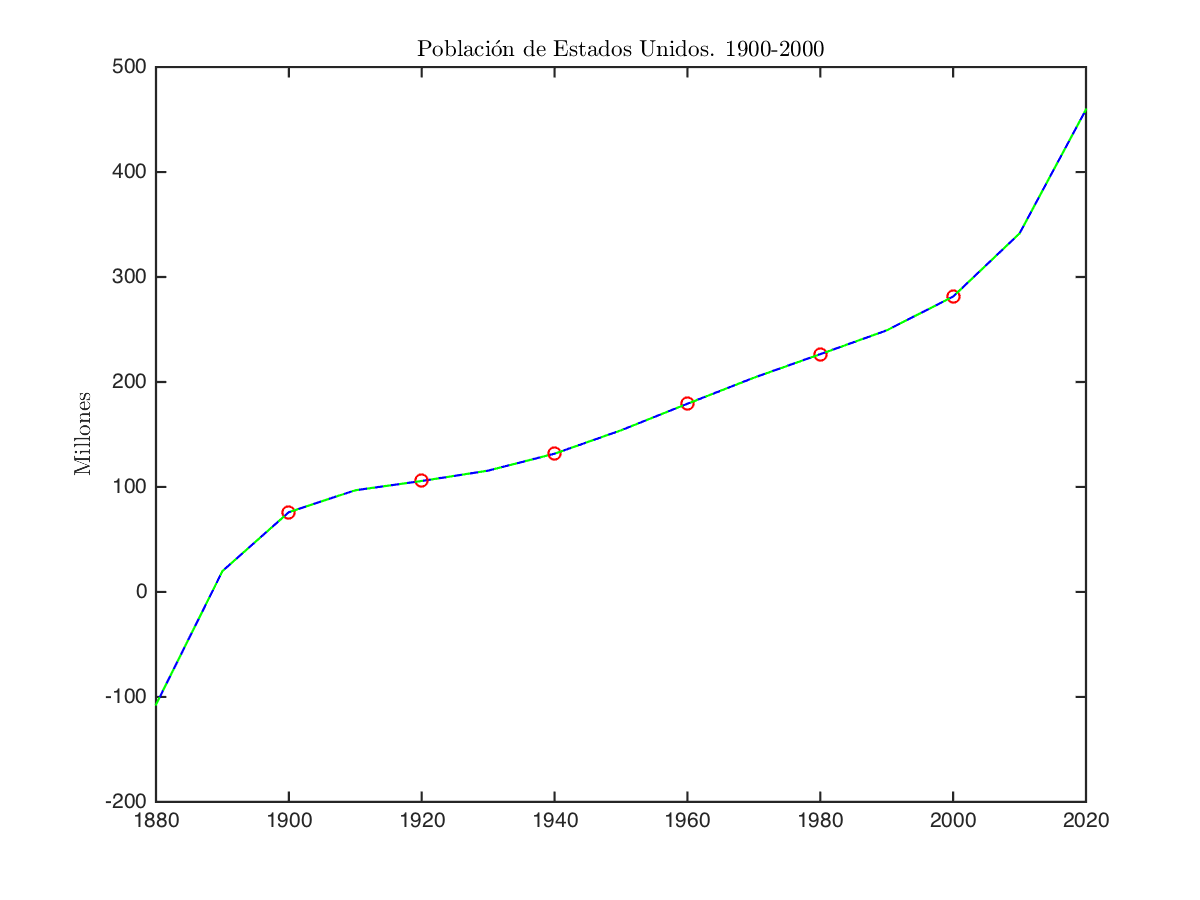
\includegraphics[scale=0.8]{data/img/populationinterplot}
	\caption{La gráfica de los puntos y los polinomios encontrados, confirma los resultados obtenidos anteriormente, primero, el comportamiento de ambos algoritmos es similar, de la misma manera, se tienen dos polinomios que incluyen los puntos de los cuales parte el polinomio resultante. Sobre la razón de este polinomio, si se compara el valor actual real con el pronosticado por el polinomio, se tiene que el valor es aproximado, si embargo, la aproximación del polinomio para valores menores a 1900, es mala, ya que por la naturaleza de la variable, este valor es positivo, y esto no se incorpora de ninguna manera al algoritmo usado.}
\end{figure}

\item Encuentre mediante cada uno de los métodos implementados el polinomio de segundo grado que pasa por los tres primeros punto en la tabla. Estime los valores de los tres puntos restantes en la tabla con estos polinomios. Compare y concluya.

\lstinputlisting[caption = {Script para comparar las predicciones realizadas, sobre un conjunto predictor de menor dimensión.}]{data/scripts/population5.m}\

$$\texttt{abserrorp1} = 0.1411042$$
$$\texttt{abserrorp2} = 0.2379690$$
$$\texttt{abserrorp3} = 0.3336886$$\

Puede verse, que al no incorporar la información de los otros años, no es posible inferir nada sobre datos fuera del rango con el cual se alimentó el algoritmo de interpolación. Esto, define que entre más datos se tenga, una mayor precisión puede tenerse.

\end{itemize}

\subsection{Implementación de algoritmos en \textsc{Matlab} (Splines)}

A continuación, se anexa la función en \textsc{Matlab}, que implementa el algoritmo para la obtención de polinomio interpolante por medio de splines cubicos con ajuste diferencial en los extremos. La metodología para este algoritmos, fue estudiada y basada en las de la referencia \cite{burden2010numerical}.

\lstinputlisting[caption = {Implementación en \textsc{Matlab} de los splines cúbicos con criterios extremos sobre las derivadas.}]{data/scripts/clamped.m}\

\subsection{Problema de aplicación (Splines)}

\begin{figure}[H]
\centering
	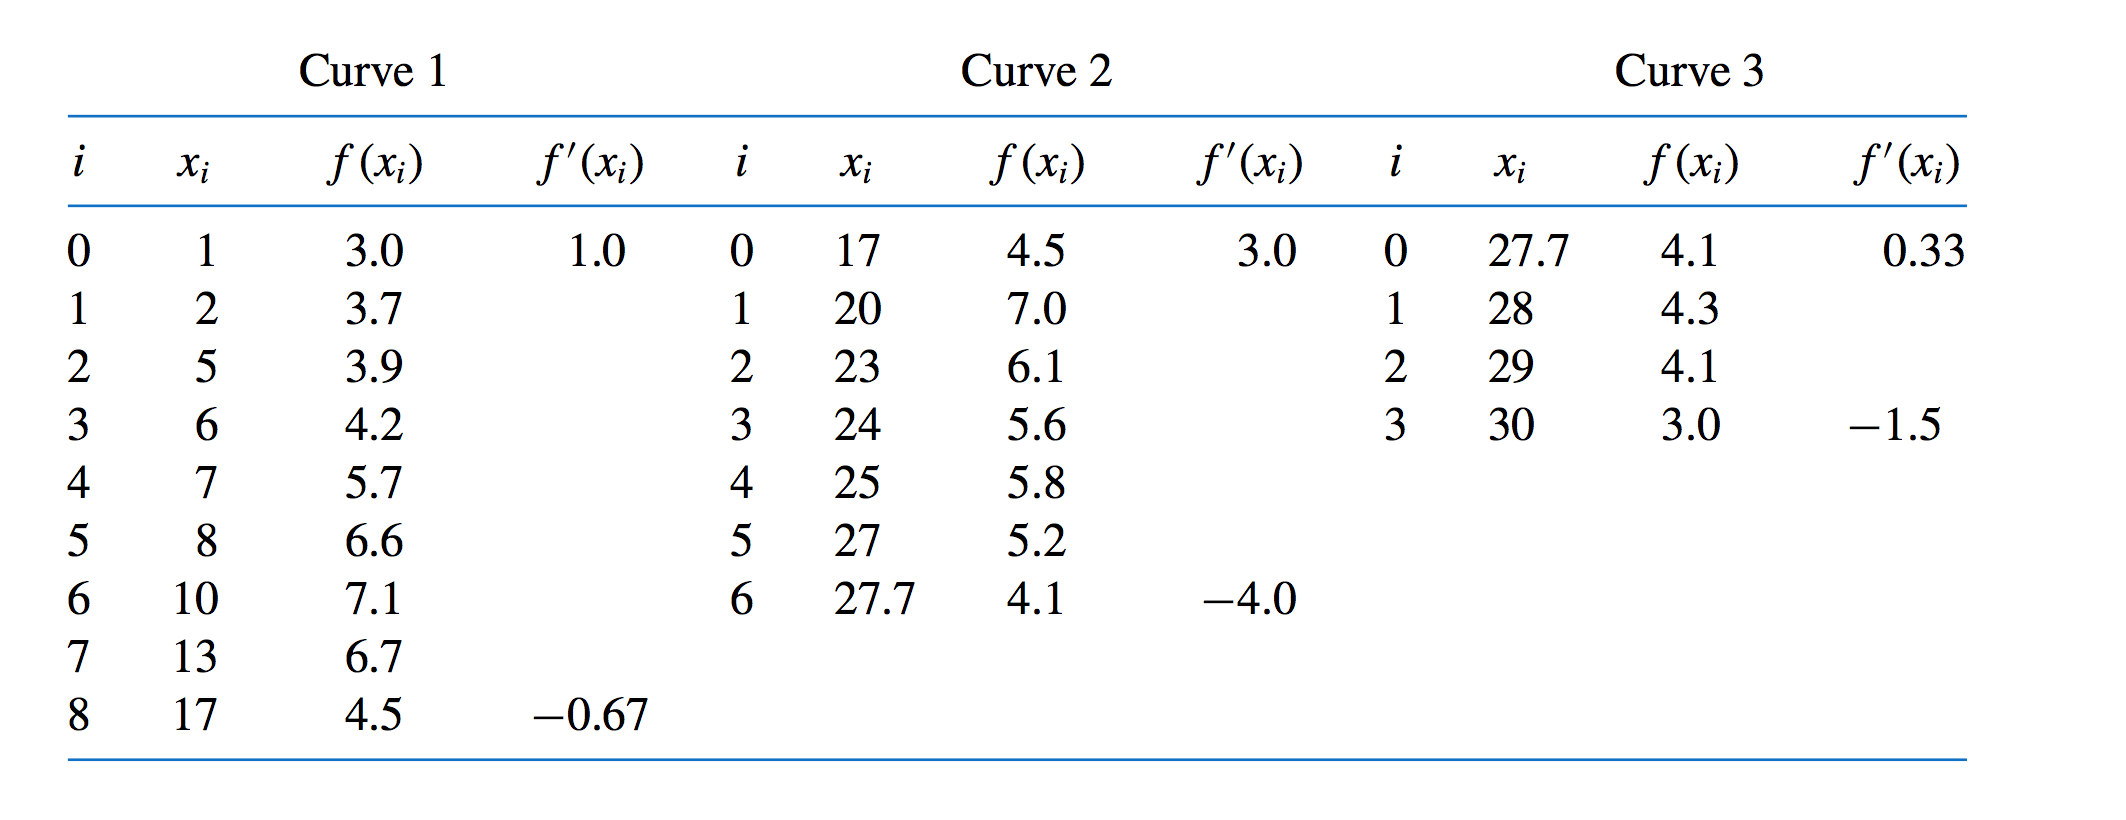
\includegraphics[scale=0.4]{data/img/snoopytable}
	\caption{}
\end{figure}

\lstinputlisting[]{data/scripts/beast.m}\

\begin{figure}[!hbt]
\centering
	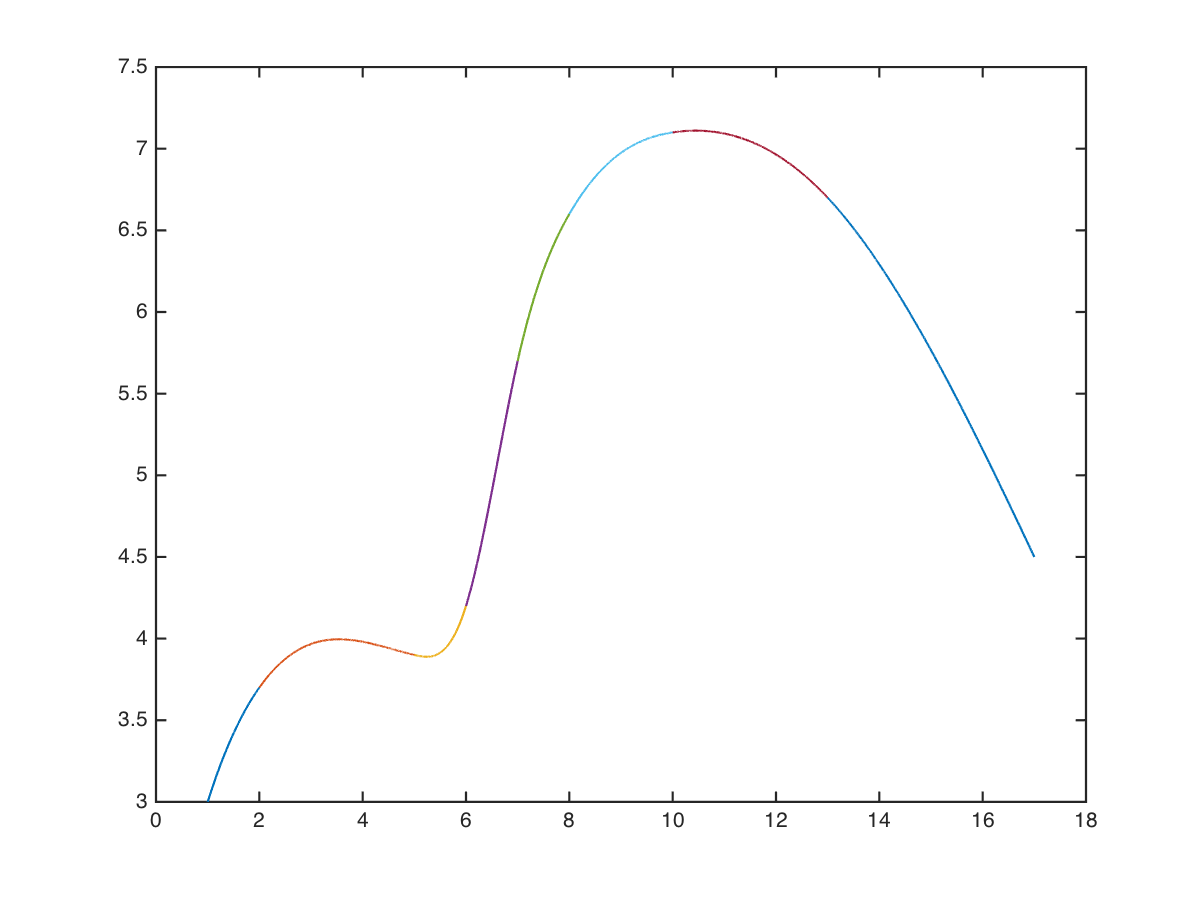
\includegraphics[scale=0.6]{data/img/curve1}
	\caption{Aproximación para la curva 1.}
\end{figure}

\begin{figure}[!hbt]
\centering
	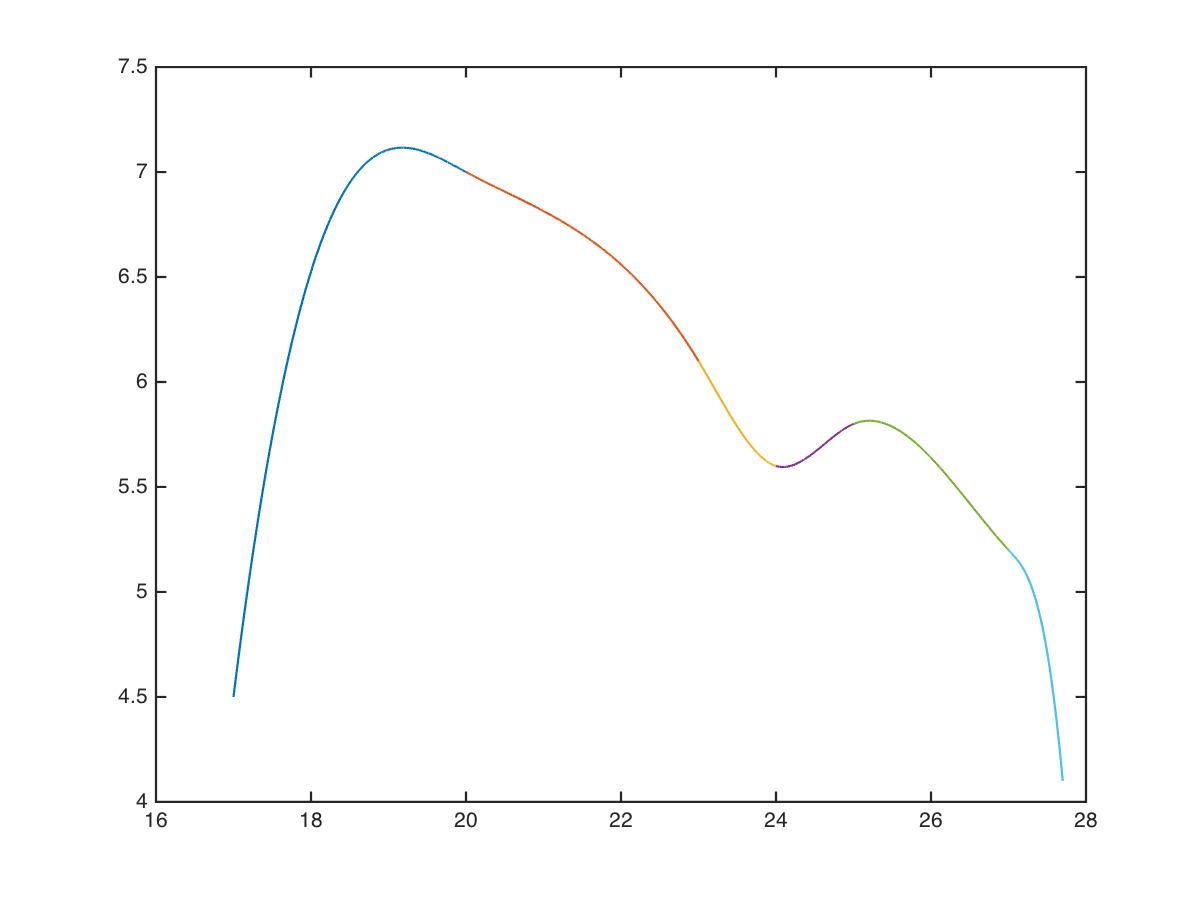
\includegraphics[scale=0.6]{data/img/curve2}
	\caption{Aproximación para la curva 2.}
\end{figure}

\begin{figure}[!hbt]
\centering
	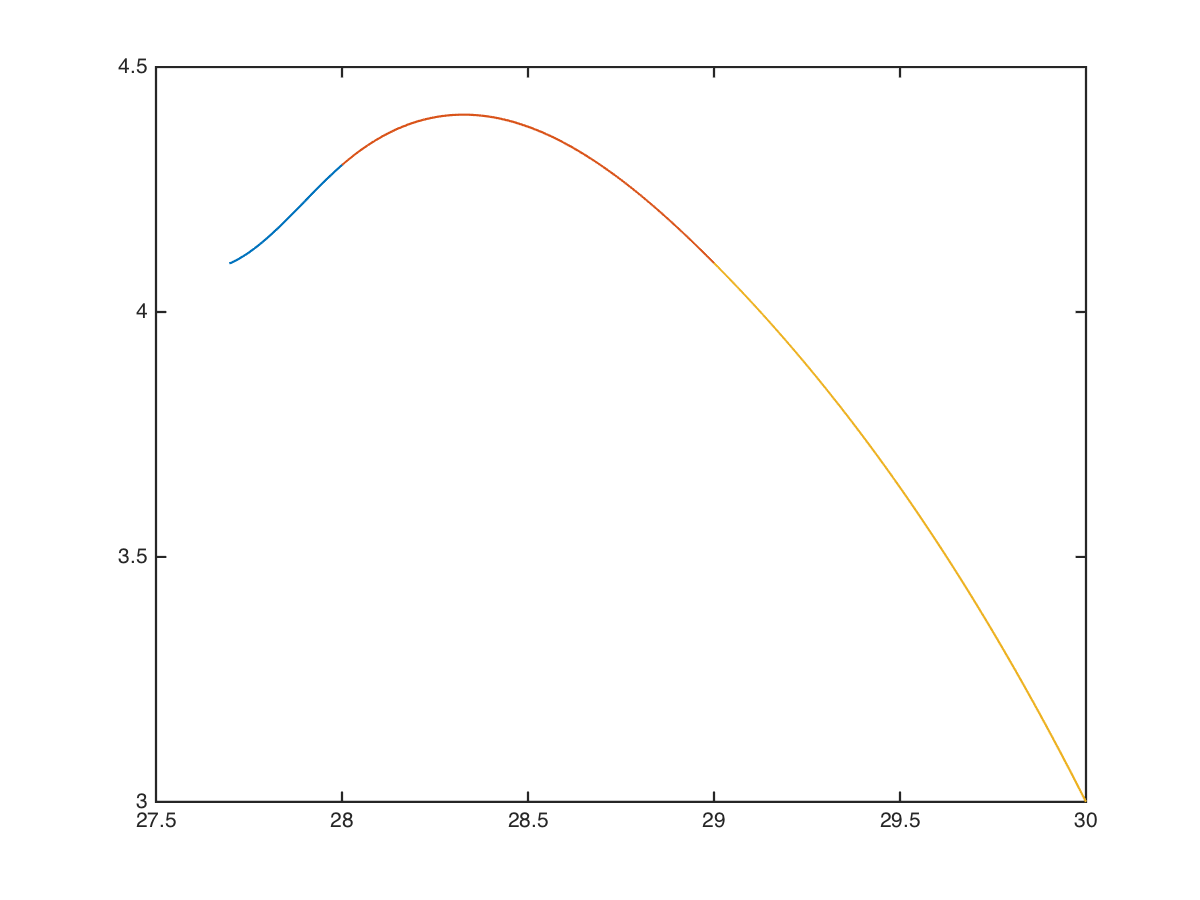
\includegraphics[scale=0.6]{data/img/curve3}
	\caption{Aproximación para la curva 3.}
\end{figure}

\begin{figure}[!hbt]
\centering
	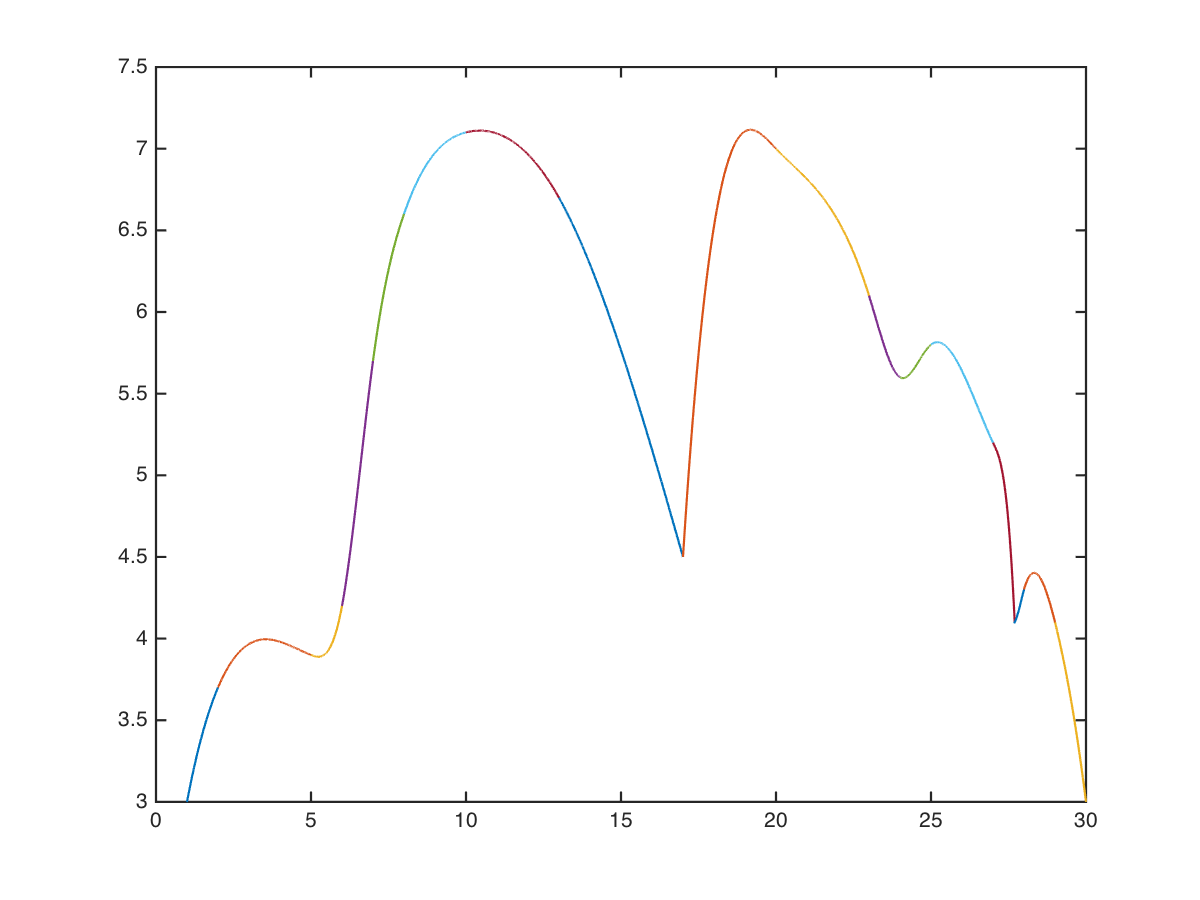
\includegraphics[scale=0.6]{data/img/beastcurve}
	\caption{Unión de las curvas anteriores, esto completa la gráfica requerida según el enunciado.}
\end{figure}


%==================================================================
\section{Conclusiones}

El desarrollo de los ejercicios propuestos para el laboratorio, sirvieron para conceptualizar los algoritmos fundamentales para la obtención de funciones analíticas a partir de una serie de datos discretos, es decir, los algoritmos para la interpolación polinomial con pares discretos de datos.  Entender estos algoritmos, sus ventajas y modos de uso, permite extender la solución de otros problemas mucho más prácticos de análisis numérico, por ejemplo, se sabe que muchos problemas en diferenciación, integración numérica, y tratamiento de ecuaciones diferenciales, se pueden aproximar por medio de polinomios sobre pares de datos discretos.\\

Por medio del desarrollo del laboratorio, se identificaron algunos de estos algoritos (Lagrange, Newton-Gregory y Splines) para el tratamiento del problema de interpolación, sobre estos, se estudió la pertinencia de uso, su exactitud, y el problema dimensional que poseen, además, se aplicaron casos prácticos de predicción y de aproximación analítica a la interpolación de ciertos datos, ajustando el algoritmo con las derivadas de los extremos. Cada uno de estos algoritmos, fueron estudiados haciendo uso de \textsc{Matlab}.
%==================================================================

\section{Bibliografía}

\begingroup
\renewcommand{\section}[2]{}%
\begin{thebibliography}{}

\bibitem{ascher2011numerical} Ascher, U. M, Greif, C. {\em A First Course in Numerical Methods.}  2011. Society for Industrial \& Applied Mathematics - Computational Science and Engineering. Página 93- 108.

\bibitem{yang2005applied} Yang, W.Y. and Cao, W. and Chung, T.S. and Morris, J. {\em Applied Numerical Methods Using MATLAB.} 2005. Wiley. Pags. 50 - 57.

\bibitem{lopez2014matlab} Lopez, C. {\em MATLAB Symbolic Algebra and Calculus Tools.} 2014. MATLAB Solutions Series - Apress. Pags. 73 - 75.

 \bibitem{bradie2006friendly} Bradie, B. {\em A Friendly Introduction to Numerical Analysis.}  2006. Pearson Prentice Hall - Featured Titles for Numerical Analysis Series. Página 150 - 174.

\bibitem{burden2010numerical} Burden, R.L. and Faires, J.D. {\em Numerical Analysis.} 2010. Cengage Learning. Pags. 105 - 160.

\end{thebibliography}
\endgroup

\bibliography{sample}

\end{document}
